\documentclass[11pt, oneside]{article}
\usepackage{amsmath}
\usepackage{color}
\usepackage{graphicx}
\usepackage{subcaption}
\usepackage{hyperref}
\usepackage{verbatim}
\usepackage{arydshln}
\hypersetup{
    colorlinks,
    citecolor=black,
    filecolor=black,
    linkcolor=black,
    urlcolor=black
}
\usepackage{listings}
\lstset{ %
basicstyle=\footnotesize,       % the size of the fonts that are used for the code
numbers=left,                   % where to put the line-numbers
numberstyle=\footnotesize,      % the size of the fonts that are used for the line-numbers
stepnumber=1,                   % the step between two line-numbers. If it is 1 each line will be numbered
numbersep=5pt,                  % how far the line-numbers are from the code
backgroundcolor=\color{white},  % choose the background color. You must add \usepackage{color}
showspaces=false,               % show spaces adding particular underscores
showstringspaces=false,         % underline spaces within strings
showtabs=false,                 % show tabs within strings adding particular underscores
frame=single,           % adds a frame around the code
tabsize=2,          % sets default tabsize to 2 spaces
captionpos=b,           % sets the caption-position to bottom
breaklines=true,        % sets automatic line breaking
breakatwhitespace=false,    % sets if automatic breaks should only happen at whitespace
escapeinside={\%*}{*)}          % if you want to add a comment within your code
}

\title{Curvilinear and flux coordinates in BOUT++}
\author{A.Smolyakov, O.Chapurin}

\begin{document}


\maketitle

\tableofcontents
\newpage

\section{Introduction}
BOUT++ \cite{dudson2009bout++} is designed to simulate arbitary number of plasma fluid equations in 3D curvilinear coordinates using finite-difference methods. It has been developed from BOUT \cite{umansky2006bout} simulation code for 2-fluid tokamak edge simulations, from where it inherited coordinate system metric tensor $g^{ij} = g^{ij}\left(x,y\right)$ (constant in one dimension). It means, it is restricted to the coordinate system with axi- or translationally symmetric geometry. Even 2D metric tensors allows the code to be used to simulate plasmas cylindrical or non-orthogonal coordinate systems such as flux coordinates for tokamak simulations.
\section{Coordinate system and operators}
To specify a coordinate system one should define each component of the metric tensors $g^{ij}$ and $g_{ij}$. Jacobian $J$ and Crystoffel symbol $\Gamma^i_{jk}$ components will be calculated from given metric tensor components, but can be specified as well. All differential operators contain these quantities. By default metric is cartesian $g^{ij} = g_{ij} = I,$ where $I$ is the identity matrix.

We can specify these quantities in either grid file or input option (BOUT.inp) file, from where they are read on a program initialization step. Another option is to define them in the physics module, which could lead to the implementation of evolving in time (space) metric tensors. As it was mentioned, our coordinate system is restricted to having one symmetry direction ($z$), so all metric tensor components are 2D fields. Note that grid spacing $dx\left(x,y\right), dy\left(x,y\right)$ are 2D fields as well, but $dz$ is a scalar, so we can work with non-uniform meshes in $x$-, $y$-directions only.

By convention $y$ coordinate is the parallel direction. Thus, we can divide differential operators into two categories: those who are independent of any coordinate system and those which assume $\mathbf{B} = \nabla z \times \nabla x$ in a Clebsch coordinate system, where $\mathbf{B}$ aligned with the $y$ coordinate. The following table contains differential operators for general coordinate system:
\newline

\begin{tabular}{| l | r |} \hline		
  Math expression & Result=Operator(Input) \\ \hline
  $\mathbf{v} = \nabla f$ & Vector = Grad(Field) \\
  $f = \nabla \cdot \mathbf{a}$ & Field = Div(Vector) \\
  $\mathbf{v} = \nabla \times \mathbf{a}$ & Vector = Curl(Vector) \\
  $f = \mathbf{a} \cdot \nabla g$ & Field = \verb|V_dot_Grad|(Vector, Field) \\
  $\mathbf{v} = \mathbf{a} \cdot \nabla \mathbf{b}$ & Vector = \verb|V_dot_Grad|(Vector, Vector) \\
  $f = \nabla^2 g$ & Field = Laplacian(Field) \\ \hline
\end{tabular}


General expression for these operators are:
\begin{equation}\label{grad}
\nabla f = \frac{\partial f}{\partial u^i} \nabla u^i,
\end{equation}

\begin{equation}\label{div}
\nabla \cdot \mathbf{A} = \frac{1}{J} \frac{\partial}{\partial u^i} \left( J \sqrt{g^{ij}} A_j \right),
\end{equation}

\begin{equation}\label{laplacian}
\nabla^2 f = G^j \frac{\partial f}{\partial u^i} + g^{ij} \frac{\partial^2 f}{\partial u^i \partial u^j},
\end{equation}

where
\begin{equation}\label{gees}
G^j = \frac1{J}\frac{\partial}{\partial u^i}\left( J g^{ij} \right).
\end{equation}


Operators which assume that the equilibrium magnetic field is written in Clebsch form are:
\newline

\begin{tabular}{| l | r |} \hline		
  Math expression & Result=Operator(Input) \\ \hline
  $\partial^0_{\parallel} = \mathbf{b}_0 \cdot \nabla$ & Scalar = \verb|Grad_par|(Scalar) \\
  $\nabla^0_{\parallel}f = B_0\partial^0_{\parallel} \left(\frac{f}{B_0}\right)$ & Scalar = \verb|Div_par|(Scalar) \\
  $\nabla^2_{\parallel}f = \nabla \cdot \mathbf{b}_0\mathbf{b}_0 \cdot \nabla f$ & Scalar = \verb|Laplace_par|(Scalar) \\
  $\nabla^2_{\perp}f = \nabla^2 f - \nabla^2_{\parallel} f$ & Field =  \verb|Laplace_perp|(Field) \\
  $f = \mathbf{b}_0 \cdot \nabla \phi \times \nabla A$ & Scalar = \verb|b0xGrad_dot_Grad|(Scalar, Scalar) \\ \hline
\end{tabular}
\newline

Here $\mathbf{B} = B_0 \mathbf{b}$ is a background equilibrium (unperturbed) magnetic field and
\begin{equation}\label{clebsch}
\mathbf{B} = \nabla z \times \nabla x = \frac1{J}\mathbf{e}_y, %\ \left| B_0 \right|= \frac{\sqrt{g_{yy}}}{J}
\end{equation}

according to Clebsch form. The unit vector $\mathbf{b}$ in the direction of equilibrium $\mathbf{B}$
\begin{equation}
\mathbf{b} = \frac1{JB_0} \mathbf{e}_y = \frac1{JB_0}\left(g_{xy}\nabla x + g_{yy}\nabla y + g_{zy}\nabla z\right)
\end{equation}


\section{Cylindrical coordinates}
The easiest way to specify cylindrical coordinates is to use a known expression for a contravariant metric tensor components
\begin{equation}\label{metric1}
g^{ij} =
\begin{pmatrix}
1 & 0 & 0 \\ 0 & 1 & 0 \\ 0 & 0 & 1 / r^2
\end{pmatrix}
\end{equation}

Due to orthogonality of cylindrical coordinates covariant form of metric tensor will be just $g_{ii} = 1 / g^{ii}, \ i = 1,2,3$. Here BOUT's $(x,y,z)$ represent a cylindrical $(r,z,\phi)$. 

\textcolor{red}{\emph{This metric tensor should also work with $(z,r,\phi)$, i.e. BOUT's $y$ is the radial direction, but I couldn't succeed with that and don't understand why. }}


\subsection{Differential operators}
Inverse Jacobian $J^{-1}$ for given coordinates can be found using metric tensor $J^{-1} = \det{g^{ij}} = 1 / r$, so $J = r$.
Using Equations (\ref{grad}, \ref{div}), a general form of these operatoes for our cylidndrical coordinates
\begin{eqnarray}
\nabla f = \frac{\partial f}{\partial r}\mathbf{e}_r + \frac{\partial f}{\partial r}\mathbf{e}_z + \frac{1}{r} \frac{\partial f}{\partial \phi}\mathbf{e}_{\phi}, \label{grad1} \\
\nabla \cdot \mathbf{A} = \frac{1}{r} \frac{\partial}{\partial r} \left( r A_r \right) + \frac{\partial A_z}{\partial z}  + \frac{1}{r} \frac{\partial A_{\phi}}{\partial \phi}. \label{div1}
\end{eqnarray}
From Eq. (\ref{gees}) we find that
\begin{eqnarray*}
G^1 = \frac{1}{r} \frac{\partial}{\partial r} \left( r \right) = \frac{1}{r}, \\
G^2 = \frac{1}{r} \frac{\partial}{\partial z} \left( r \right) = 0, \\
G^3 = \frac{1}{r} \frac{\partial}{\partial \phi} \left( r \frac1{r} \right) = 0.
\end{eqnarray*}
Finally, we have the general expression for Laplacian operator from Eq.(\ref{laplacian})
\begin{equation}\label{laplacian1}
\nabla^2 f = \frac{1}{r}\frac{\partial f}{\partial r} + \frac{\partial^2 f}{\partial r^2} + \frac{\partial^2 f}{\partial z^2} + \frac{1}{r^2} \frac{\partial^2 f}{\partial \phi^2}.
\end{equation}

\subsection{Verification with BOUT++}
To verify this method a simple heat conduction problem was implemented\footnote{More details (animation, source files) can be found in https://github.com/alxmar/conduction-cylinder} and solved
\begin{equation}\label{conduction}
\frac{\partial T}{\partial t} = \chi \nabla^2 T,
\end{equation}
with a following input options for geometry, according to metric tensor (\ref{metric1})
\begin{lstlisting}
[mesh]  # Mapping to cylinder: x -> r,  y -> z,  z -> phi

nx = 68 # including 2*2 guard points
ny = 1

Rmin = 0.05
Rmax = 1.8

Rxy = Rmin + (Rmax - Rmin)*x   # Rxy = [Rmin, ..., Rmax]
dr = (Rmax - Rmin) / (nx-4)    # 2 guard points on each side

Lz = 1.0
dx = dr
dy = 1.0

### Contravariant metric tensor components
g11 = 1.0
g22 = 1.0
g33 = 1.0/Rxy^2

### Covariant metric tensor components
g_11 = 1 / g11
g_22 = 1 / g22
g_33 = 1 / g33
\end{lstlisting}

The analytical solution to this two-dimensional cylindrical $(r,\phi)$ problem with Neumann boundary conditions is:
\begin{equation}
T\left(r,\phi,t\right) = \sum\limits_{m=0}^{\infty}\sum\limits_{k=1}^{\infty} A_{m,k} J_m\left(\frac{B_{m,k}r}{r_0}\right) \cos\left(m\phi\right) \exp\left( -\chi \frac{B_{m,k}^2}{r_0^2}t\right) + C,
\end{equation}
where $B_{m,k}$ is the $k^{\text{th}}$ zero of the function $J^{'}_m(r), \ C$ is arbitary constant.
With the intial condition $T_0(r,\phi, t = 0) = \cos(2\phi)$ (Fig.\ref{fig1}) the solution is simplified to\cite{ma2015macro}
\begin{equation}
T\left(r,\phi,t\right) = \sum\limits_{k=1}^{20} A_{2,k} J_2\left(\frac{B_{2,k}r}{r_0}\right) \cos\left(2\phi\right) \exp\left( -\chi \frac{B_{2,k}^2}{r_0^2}t\right),
\end{equation}
where we can take first 20 terms of the infinite sum. Solving Eq.(\ref{conduction}) in BOUT++ with a clyndrical metric components, presented above, we can see that the numerical and analytical results are highly consistent (Fig.\ref{fig:naive}).
\begin{figure}
	\centering
	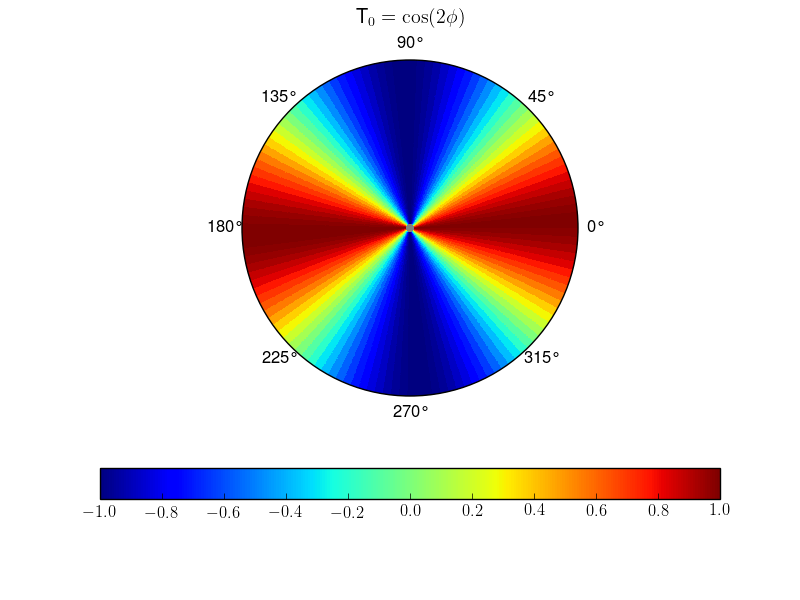
\includegraphics[width=1.\linewidth]{pics/tempBR00000.png}
	\caption{Plot in the polar coordinates of the initial condition for the 2-D heat conduction equation, $T_0(r,\phi, t = 0) = \cos(2\phi), n_r = 64, n_{\phi} = 128.$}
	\label{fig1}
\end{figure}

\begin{figure}
\centering
\begin{subfigure}{.5\textwidth}
  \centering
  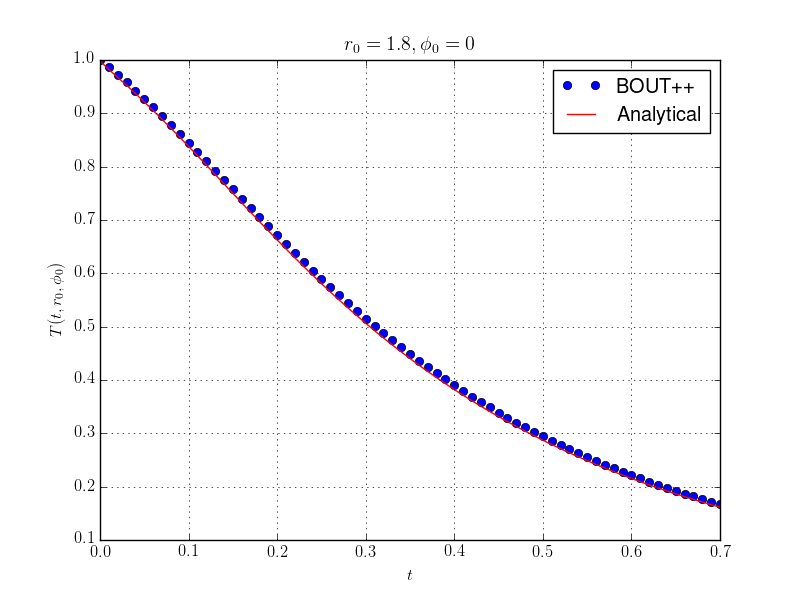
\includegraphics[width=1.\linewidth]{pics/cmpr-1.png}
  \caption{}
  \label{fig:sub1}
\end{subfigure}%
\begin{subfigure}{.5\textwidth}
  \centering
  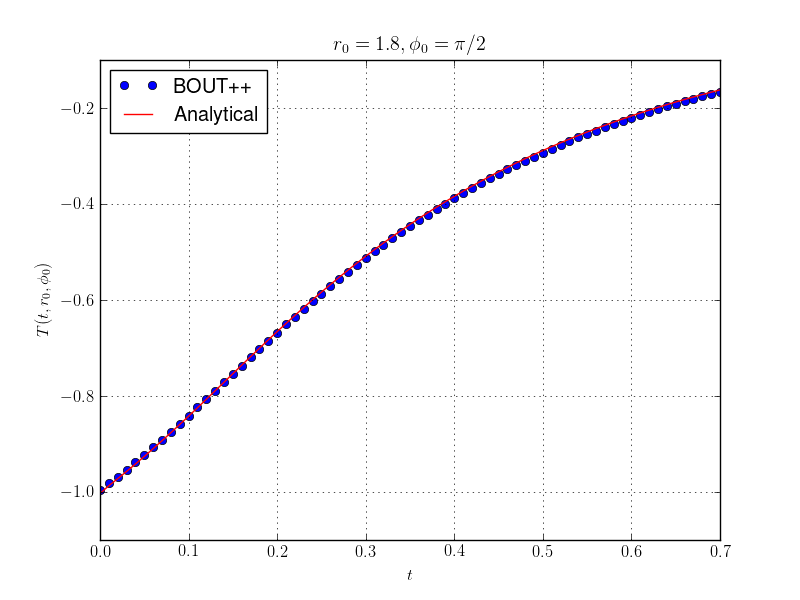
\includegraphics[width=1.\linewidth]{pics/cmpr-2.png}
  \caption{}
  \label{fig:sub2}
\end{subfigure}
\caption{The comparsion between simulation results from BOUT++ and the analytical solution at two different positions}
\label{fig:naive}
\end{figure}

\newpage
\section{Cylindrical flux coordinates}
\subsection{Axial constant magnetic field (LAPD without
mirrors)}

Here we introduce an orthogonal cylindrical coordinate system $(\psi, z, \phi)$, where $\psi$ is the axial flux, $z$ is the axial coordinate, $\phi$ the azimuthal angle (from $0$ to $2 \pi$). Clebsch form (\ref{clebsch}) for megnetic field implies that
\begin{equation*}
\mathbf{B} =\nabla \phi \times \nabla \psi
\end{equation*}%
Chosing a magnetic flux to be $\psi = B_0 r^2 / 2$, where $r$ is the radial coordinate in the standard cylindrical coordinates, we obtain the axial constant magnetic field $\mathbf{B} = B_0 \mathbf{e}_z$.
The contravariant metric tensor is defined as 
\begin{equation}
g^{ij}\equiv \mathbf{e}^{i}\cdot\mathbf{e}^{j}=\nabla u^{i}\cdot \nabla u^{j},
\end{equation}
where unit vectors for our coordinates are
\begin{eqnarray}
\mathbf{e}^{\psi} &\equiv& \nabla \psi = B_{0}r\mathbf{\hat{e}_{r}}, \\
\mathbf{e}^{z} &\equiv& \nabla z = \mathbf{\hat{e}_{z}}, \\
\mathbf{e}^{\phi} &\equiv& \nabla \phi = \frac{1}{r}\mathbf{\hat{e}_{\phi }},
\end{eqnarray}%

Therefore we have 
\begin{equation*}
g^{ij}=\left(
\begin{array}{ccc}
\left( B_{0}r\right) ^{2} & 0 & 0 \\
0 & 1 & 0 \\
0 & 0 & 1/r^{2}%
\end{array}%
\right)
\end{equation*}%
and a covariant form
\begin{equation*}
g_{ij}=\left(
\begin{array}{ccc}
1/\left( B_{0}r\right) ^{2} & 0 & 0 \\
0 & 1 & 0 \\
0 & 0 & r^{2}%
\end{array}%
\right)
\end{equation*}

\subsubsection{Differential operators}
\emph{(this subsubsection is not finished)}


The Jacobian is found to be constant $J = B_0$.

Laplacian operator in general is given by
\begin{eqnarray*}
\nabla ^{2}F &=&\frac{1}{J}\frac{\partial }{\partial u^{i}}\left( Jg^{ij}%
\frac{\partial F}{\partial u^{j}}\right) =\frac{\partial }{\partial x^{B}}%
\left( g^{xx}\frac{\partial F}{\partial x^{B}}\right) +\frac{\partial }{%
\partial y^{B}}\left( g^{yy}\frac{\partial F}{\partial y^{B}}\right) +\frac{%
\partial }{\partial z^{B}}\left( g^{zz}\frac{\partial F}{\partial z^{B}}%
\right) \\
&=&\frac{\partial }{\partial x^{B}}\left( B_{0}^{2}r^{2}\frac{\partial F}{%
\partial x^{B}}\right) +\frac{\partial }{\partial y^{B}}\left( \ \frac{%
\partial F}{\partial y^{B}}\right) +\frac{\partial }{\partial z^{B}}\left(
\frac{1}{r^{2}}\frac{\partial F}{\partial z^{B}}\right) \\
&=&\frac{\partial }{\partial \psi }\left( B_{0}^{2}r^{2}\frac{\partial F}{%
\partial \psi }\right) +\frac{\partial }{\partial z}\left( \ \frac{\partial F%
}{\partial z}\right) +\frac{\partial }{\partial \phi }\left( \frac{1}{r^{2}}%
\frac{\partial F}{\partial \phi }\right) \\
&=&\frac{1}{r}\frac{\partial }{\partial r }\left( r\frac{\partial F}{%
\partial r}\right) +\frac{\partial }{\partial z}\left( \ \frac{\partial F%
}{\partial z}\right) +\frac{\partial }{\partial \phi }\left( \frac{1}{r^{2}}%
\frac{\partial F}{\partial \phi }\right),
\end{eqnarray*}
where we have used a transformation
\begin{equation*}
\frac{\partial}{\partial \psi} = \frac{1}{B_0 r} \frac{\partial}{\partial r}.
\end{equation*}
Therefore, it becomes a standard Laplacian operator in cylindrical coordinates.


\subsubsection{Verification with BOUT++}
\begin{equation}
\frac{\partial T}{\partial t} = \chi \nabla^2 T
\end{equation}
with the input file:

\begin{lstlisting}
[mesh]  # Mapping: x -> r,  y -> z,  z -> phi


nx = 36
ny = 1

#hthe = 3.0
Rmin = 0.05
Rmax = 1.8

Rxy = Rmin + (Rmax - Rmin)*x   # Rxy = [Rmin, ..., Rmax]
dr = (Rmax - Rmin) / (nx-4)

Bxy = 1.
Ly = 3.0
dy = 1.
dx = Bxy*Rxy*dr # Required by definition of flux psi = Bxy*r^2/2

### Contravariant metric tensor components
g11 = (Bxy*Rxy)^2
g22 = 1.0
g33 = 1./(Rxy)^2

### Covariant metric tensor components
g_11 = 1 / g11
g_22 = 1 / g22
g_33 = 1 / g33

J = Bxy
\end{lstlisting}
Intial conditions and other parameters were identical to the heat conduction problem in the previous section. Results are presented in Fig.(\ref{fig2}).
\begin{figure}
\centering
\begin{subfigure}{.5\textwidth}
  \centering
  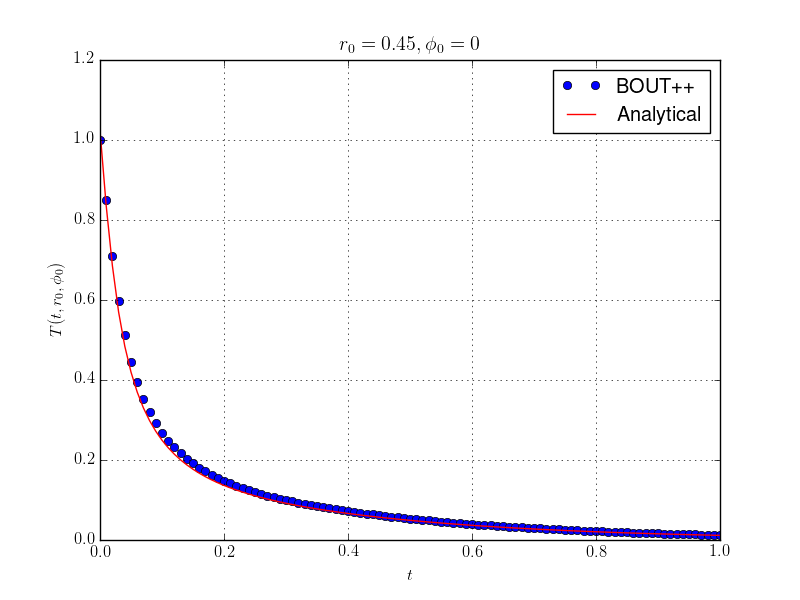
\includegraphics[width=1.\linewidth]{pics/flux-cmpr-1.png}
  \caption{}
  \label{fig:sub11}
\end{subfigure}%
\begin{subfigure}{.5\textwidth}
  \centering
  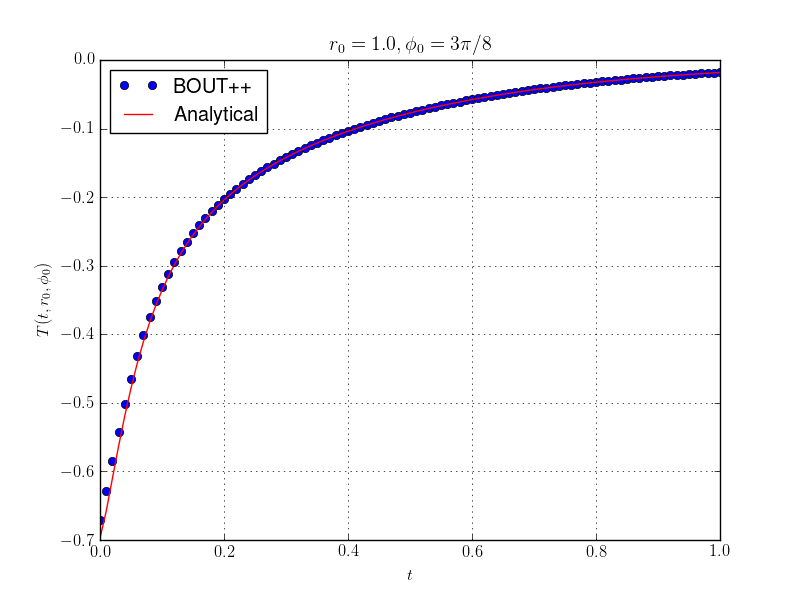
\includegraphics[width=1.\linewidth]{pics/flux-cmpr-2.png}
  \caption{}
  \label{fig:sub12}
\end{subfigure}
\caption{The comparsion between simulation results from BOUT++ and the analytical solution at two different positions}
\label{fig2}
\end{figure}

\subsection{Radial constant magnetic field}
Here we introduce an orthogonal cylindrical coordinate system $(\psi, r, \phi)$, where $\psi$ is the radial flux, $r$ is the radial coordinate, $\phi$ the azimuthal angle (from $0$ to $2 \pi$). Clebsch form (\ref{clebsch}) for megnetic field implies that
\begin{equation*}
\mathbf{B} =\nabla \phi \times \nabla \psi
\end{equation*}%
Chosing a magnetic flux to be $\psi = B_0 z$, where $z$ is the axial coordinate in the standard cylindrical coordinates, we obtain the radial constant magnetic field 
\begin{equation}
\mathbf{B} = \frac{B_0}{r} \mathbf{e}_r.
\end{equation}

Unit vectors for our coordinates are
\begin{eqnarray}
\mathbf{e}^{\psi} &\equiv& \nabla \psi = B_{0}\mathbf{e}_z, \\
\mathbf{e}^{z} &\equiv& \nabla r = \mathbf{e}_r, \\
\mathbf{e}^{\phi} &\equiv& \nabla \phi = \frac{1}{r}\mathbf{e}_{\phi},
\end{eqnarray}%

Therefore we have
\begin{equation*}
g^{ij}=\left(
\begin{array}{ccc}
B_{0}^{2} & 0 & 0 \\
0 & 1 & 0 \\
0 & 0 & 1/r^{2}%
\end{array}%
\right)
\end{equation*}%
and a covariant form
\begin{equation*}
g_{ij}=\left(
\begin{array}{ccc}
1/B_{0}^{2} & 0 & 0 \\
0 & 1 & 0 \\
0 & 0 & r^{2}%
\end{array}%
\right)
\end{equation*}

\textcolor{red}{\emph{With $B_0 = 1$ this metric tensor appeared to be the same as in (\ref{metric1}), but here we have BOUT's $x$ representing $z$, and we know that it is working, but for $(r,z,\phi)$, as it was shown. Even dimensions of $\psi ~ B_0 z$ are not magnetic flux dimensions, so proabably this is wrong.}}

\subsubsection{Verification with BOUT++}
\begin{equation}
\frac{\partial T}{\partial t} = \chi \nabla^2 T
\end{equation}
with the input file:
\begin{lstlisting}
[mesh]  # Mapping to cylinder: x -> z,  y -> r,  z -> phi

nx = 5 # including 2*2 ghost points
ny = 128

Rmin = 0.05
Rmax = 1.8

Rxy = Rmin + (Rmax - Rmin)*y/(2*pi)   # as y is normalized to 0, 2*pi
dr = (Rmax - Rmin) / ny

Bxy = 1.
Ly = 2*pi
dx = Ly/ny
dy = dr

### Contravariant metric tensor components
g11 = 1.0
g22 = 1.0
g33 = 1.0/Rxy^2

### Covariant metric tensor components
g_11 = 1 / g11
g_22 = 1 / g22
g_33 = 1 / g33
\end{lstlisting}

Intial conditions and other parameters were identical to the heat conduction problem in the previous section. Results are presented in Fig.(\ref{fig3}).
\begin{figure}
\centering
\begin{subfigure}{.5\textwidth}
  \centering
  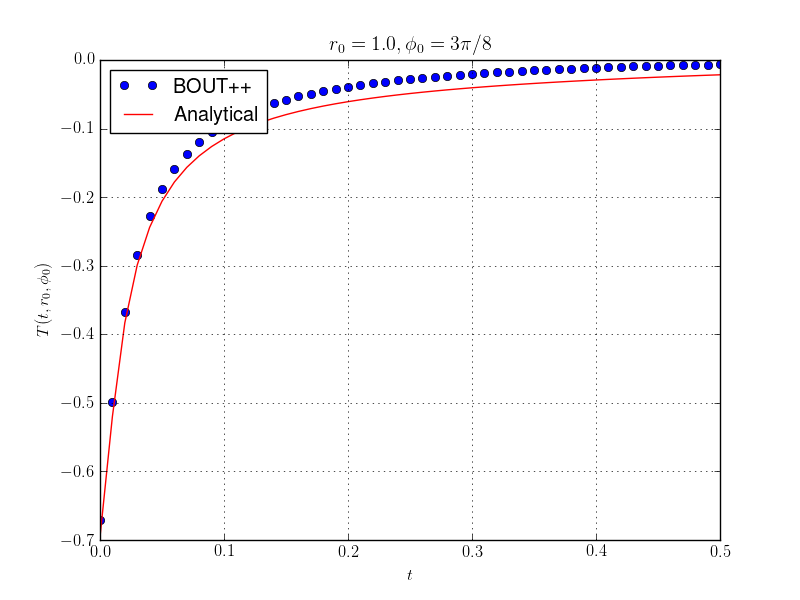
\includegraphics[width=1.\linewidth]{pics/rad-cmpr-1.png}
  \caption{}
  \label{fig:sub21}
\end{subfigure}%
\begin{subfigure}{.5\textwidth}
  \centering
  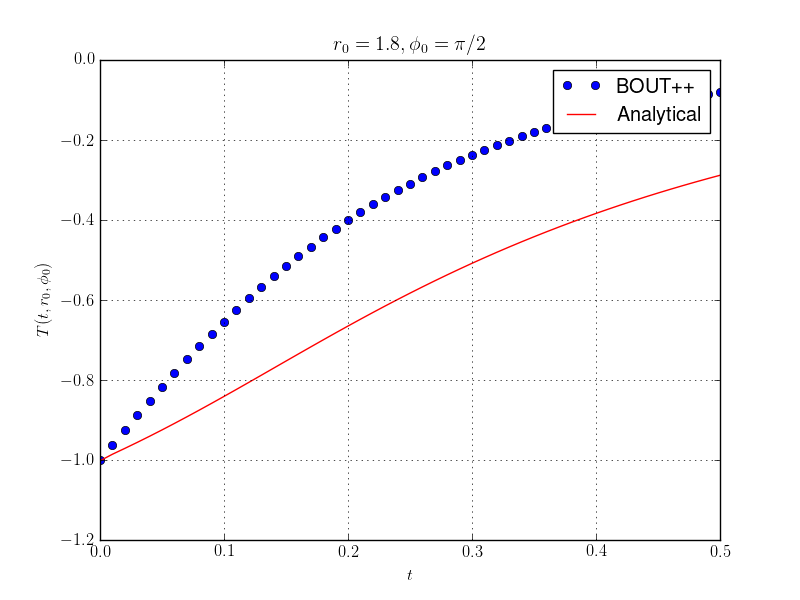
\includegraphics[width=1.\linewidth]{pics/rad-cmpr-2.png}
  \caption{}
  \label{fig:sub22}
\end{subfigure}
\caption{The comparsion between simulation results from BOUT++ and the analytical solution at two different positions}
\label{fig3}
\end{figure}



\bibliography{mybib}{}
\bibliographystyle{plain}

\end{document}



